%-------------------------------------------------------------------------------
% yum_vector_control
%-------------------------------------------------------------------------------
%
% \file        yum_vector_control.tex
% \library     Documents
% \author      Chris Ahlstrom
% \date        2015-10-24
% \update      2017-03-04
% \version     $Revision$
% \license     $XPC_GPL_LICENSE$
%
%     Provides the concepts NRPNs and vector control.  And effects.
%
%-------------------------------------------------------------------------------

\section{Vector Control}
\label{sec:vector}

   This section comes from the source-code documentation file
   \texttt{doc/Vector\_Control.txt}.
   Also see 
   \sectionref{subsubsec:stock_settings_elements_automation}, for a discussion
   of vector automation, and
   \sectionref{subsec:vector_dialogs}, for a discusson of the vector
   configuration dialog.

   Vector load and save also work from the command-line, for a complete vector
   set, with all mappings, instruments, etc.
   One can independently decide which
   channel to load and save from, so one can actually build up a vector set in
   (say) channel 3, then later decide to use it in channel 7.
   The vector settings file
   \index{vector! settings file}
   has the extension \texttt{.xvy} standing for 
   \textsl{Xml / Vector / Yoshimi}.

   Vector controls can be set on any and all channels,
   stored in both patch sets and saved state.

\subsection{Vector / Basics}
\label{subsection:vector_basics}

   Vector control is a way to control more than one part with the controllers.
   It is a little bit reminiscent of the "vector" control knob on the Yamaha
   PSS-790 consumer MIDI synthesizer.  Vector control is only possible if one
   has 32 or 64 parts active.  Setup is per MIDI channel, so one can have
   totally different vector behaviour on, say, channel 1 and channel 5.
   \index{vector!base channel} The term \textsl{base channel} refers to the
   incoming MIDI channel that a particular vector setup will respond to, and
   the base channel directly relates to the 1 to 16 range of parts in the mixer
   panel.

   Vector control has been extended so that there are four independent
   'features' that each axis can control. One is fixed as \textsl{Volume} (if
   enabled) but the other three can be any valid CC, and can also be reversed.
   The vector 'sweep' CCs are split out very early in the MIDI chain, and the
   new CCs created are fed back in before any other processing. The result of
   this is that once we eventually get MIDI-learn implemented, the control
   possibilities will expand dramatically.

   In vector mode parts will still play together but the vector controls can
   change their volume, pan, filter cutoff in pairs, controlled by user-defined
   CCs set up with NRPNs.

   One must set the X axis CC before the Y axis, but if one doesn't set the Y
   axis at all, one can run just a single axis.  If one has only 32 parts
   active, Y settings are ignored.  One cannot make any Y axis settings until,
   at the very least, the X CC has be set, and if one sets that back to zero,
   the Y axis is again disabled.  Setting an X axis control CC will immediately
   enable the base channel part and the part number + 16, as well as setting
   \textsl{Yoshimi} for 32 parts, if it was less than that. If it was the same,
   or was set to 64 parts, then nothing changes. Setting the CC will also
   ensure that both parts are actually responding to that MIDI channel (they
   might have been set to something else, or even disabled).

   Setting a Y axis control CC will immediately enable the part (base channel +
   32) and the part number + 48, as well as setting for 64 parts, if it was
   less than that. If it was the same, again nothing changes, and again the
   parts are set to the correct MIDI channel.

   The instruments that are loaded into the respective parts are always shown,
   regardless of whether there is a configured vector or not. They are a direct
   analogue of the main part instrument selector and behave in the same way
   (i.e.  click on them to open the instrument selection window).  There are
   tooltips for these items, along with the base channel and controller.

   The features are pretty self descriptive as soon and you click on them. They
   apply inversely to the \textsl{pair} of instruments on each axis.  One could
   have all four if One wanted to, but it would probably sound messmessy

   Options are pretty obvious, and follow a familiar pattern for load, save,
   etc.  Loading or saving a vector will put the leafname in the bottom text
   field.

   Disabling or clearing vectors will \textsl{not} change the number of parts
   because they may have already been set to increased numbers for some other
   purpose.  Similarly, disabling or clearing vectors will \textsl{not} clear
   any instrument patches that have been loaded.
   Of course making any changes to the parts outside vector control will likely
   mess them up. It won't do any harm, just be puzzling.

   For example:
   parts 1 and 17 can be set as x1 \& x2 (volume only) while parts 33 and 49
   can be y1 \& y2 (pan only).

   Independently of this Parts 2 \& 18 could use filter and pan from another
   CC.

\subsection{Vector Dialogs}
\label{subsec:vector_dialogs}

   Vectors provide a way of mixing up to four parts in a manner that can be
   automatec, saved, and loaded.  The features of vector control are presented
   in \sectionref{sec:vector}.
   Vector setup and control from the \textsl{Yoshimi} command-line are
   discussed in
   \sectionref{subsec:command_line_command_level}.
   Here, we discuss the vector configuration dialog.
   (As an exercise, one can compare the various functions of the vector dialog
   to the command-line commands one can use to set up the vector
   functionality.)
   The new \textbf{Yoshimi / Vectors} menu entry brings up the following
   dialog:

\begin{figure}[H]
   \centering 
%  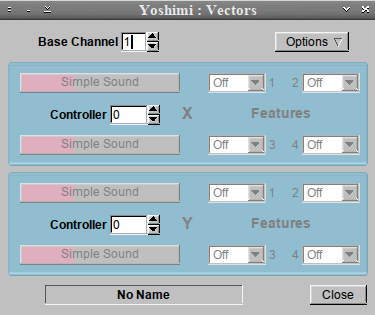
\includegraphics[scale=0.75]{1.4.0/yoshimi-vectors-dialog.png}
   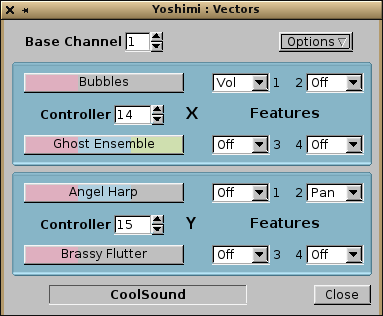
\includegraphics[scale=0.75]{1.4.1/Vectors.png}
   \caption{Yoshimi Vectors Dialog}
   \label{fig:yoshimi_vectors_dialog}
\end{figure}

   The user-interface items in the vector dialog are:

   \begin{enumber}
      \item \textbf{Top Line}
      \begin{enumber}
         \item \textbf{Base Channel}
         \item \textbf{Options}
      \end{enumber}
      \item \textbf{X Vector}
      \begin{enumber}
         \item \textbf{Controller} (CC Event)
         \item \textbf{Part 1}
         \item \textbf{Part 2}
         \item \textbf{Features}
         \begin{enumber}
            \item \textbf{Feature 1} (Volume)
            \item \textbf{Feature 2} (Pan)
            \item \textbf{Feature 3} (Brightness)
            \item \textbf{Feature 4} (Modulation)
         \end{enumber}
      \end{enumber}
      \item \textbf{Y Vector}
      \begin{enumber}
         \item \textbf{Controller} (CC Event)
         \item \textbf{Part 1}
         \item \textbf{Part 2}
         \item \textbf{Features}
         \begin{enumber}
            \item \textbf{Feature 1} (Volume)
            \item \textbf{Feature 2} (Pan)
            \item \textbf{Feature 3} (Brightness)
            \item \textbf{Feature 4} (Modulation)
         \end{enumber}
      \end{enumber}
      \item \textbf{Bottom Line}
      \begin{enumber}
         \item \textbf{Vector Name}
         \item \textbf{Close}
      \end{enumber}
   \end{enumber}

   Although they are nested, for simplicity we will discuss the unique items
   serially.

   \setcounter{ItemCounter}{0}      % Reset the ItemCounter for this list.

   \itempar{Base Channel}{Vectors!base channel}
   Vector Base Channel.
   This item specifies the MIDI channel on which the vector (of parts) will be
   based.  This channel is the incoming MIDI channel to which the vector setup
   will respond to on all parts.

   Values: \texttt{1 to 16, 1*}

   \itempar{Options}{Vectors!options}
   Vector Options.

   Values: \texttt{1 to 127, 64*}

\begin{figure}[H]
   \centering 
   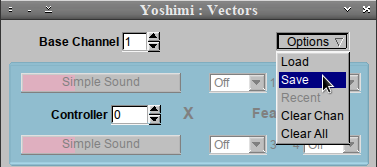
\includegraphics[scale=0.75]{1.4.0/yoshimi-vectors-options.png}
   \caption{Yoshimi Vectors Options}
   \label{fig:yoshimi_vectors_options}
\end{figure}

   The menu entries provide the actions described in this list:

   \begin{enumber}
      \item \textbf{Load}.
         Brings up a file dialog that let's one pick an arbitary vector file
         (extension \texttt{.xvy}) in an arbitrary directory, or select a
         "Favorites" directory in which to look for vector files.
         The base name of the file is then shown in the \textbf{Vector Name}
         field.
      \item \textbf{Save}.
         Brings up a file dialog that let's one save an arbitary vector file
         (extension \texttt{.xvy}) in an arbitrary directory, or select a
         "Favorites" directory in which to save a vector file.
         The base name of the file is then shown in the \textbf{Vector Name}
         field.
      \item \textbf{Recent}.
         Brings up a short list of the previous vector files dealt with.
      \item \textbf{Clear Chan}.
         Clears the base channel number????
      \item \textbf{Clear All}.
         Clears out the full vector setup, rendering it an "empty" vector setup
         that cannot be saved.
   \end{enumber}

   \index{soft load}
   Note that loading vectors is a 'soft' load. It first runs down the overall
   volume (over about 100 ms), then mutes the whole synth before performing
   the load operation. Only when that is complete does it unmute the synth. 

   \itempar{X Vector}{Vectors!x}
   The X Vector.
   This vector provides the minimal setup for a vector.  This setup requires
   \textsl{Yoshimi} to be configured for 32 parts, to be able to fully support
   a two-part vector for every MIDI channel.  This section is disabled until
   selects a \textbf{Controller} event value for it.

   \itempar{Controller}{Vectors!controller}
   Vector Controller CC Event.
   If 0, the section (\textbf{X} or \textbf{Y}) that this value is in is
   disabled.  Otherwise, the number is the MIDI continuous controller (CC)
   event value that is to be used to control the mix of the two parts involved
   in this vector.

   Values: \texttt{1 to 119, 0*}

   \itempar{Part 1}{Vectors!part 1}
   Part 1.
   The top button in the section (\textbf{X} or \textbf{Y}) selects the first
   part to use in the two-part vector.  Clicking this button brings up the
   default bank dialog.  This dialog allows one to select a part (instrument),
   or to select an different bank from which to choose a part (instrument).

   \itempar{Part 2}{Vectors!part 2}
   Part 2.
   The bottom button in the section (\textbf{X} or \textbf{Y}) selects the
   second part to use in the two-part vector.  Clicking this button brings up
   the default bank dialog, just as for the \textbf{Part 1} button.

   \itempar{Feature 1}{Vectors!volume}
   Vector Feature 1, Volume.
   This feature can be disabled, or enabled.  Feature 1 is always fixed as MIDI
   event 7 (volume), and is not reversible.
   When enabled, the volume is traded off between the first part and second part
   as the selected MIDI CC controller event data value changes.
   While the first part increases in volume, the second part decrease in
   volume, and vice versa.

\begin{figure}[H]
   \centering 
   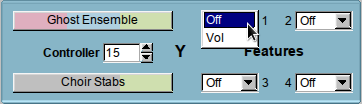
\includegraphics[scale=0.75]{1.4.0/yoshimi-vectors-feature-1.png}
   \caption{Yoshimi Vectors, Feature 1}
   \label{fig:yoshimi_vectors_feature_1}
\end{figure}

   Values: \texttt{Off*, Vol}

   Note that the common theme between all features is that they apply inversely
   to the two parts/instruments that are paired in an \textbf{X}
   or \textbf{Y} vector.

   \itempar{Feature 2}{Vectors!pan}
   Vector Feature 2, Pan.
   This feature can be disabled, enabled, or reversed.
   When enabled, it acts similarly to volume, panning from left to right as the
   data value increases.
   When reversed, it pans from right to left as the data value increases.

\begin{figure}[H]
   \centering 
   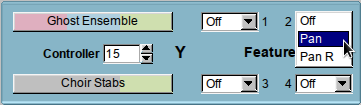
\includegraphics[scale=0.75]{1.4.0/yoshimi-vectors-feature-2.png}
   \caption{Yoshimi Vectors, Feature 2}
   \label{fig:yoshimi_vectors_feature_2}
\end{figure}

   Values: \texttt{Off*, Pan, Pan R}

   \itempar{Feature 3}{Vectors!brightness}
   Vector Feature 3, Brightness.
   Brightness here refers to the application of a (we presume) low-pass filter
   with a varying cutoff frequency.
   This feature can be disabled, enabled, or reversed.
   When enabled, it acts similarly to volume, changing the brightness
   from left to right as the data value increases.
   When reversed, it changes the brightness from right to left as the data
   value increases.

\begin{figure}[H]
   \centering 
   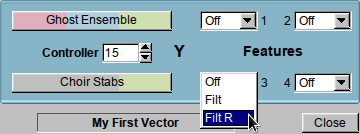
\includegraphics[scale=0.75]{1.4.0/yoshimi-vectors-feature-3.png}
   \caption{Yoshimi Vectors, Feature 3}
   \label{fig:yoshimi_vectors_feature_3}
\end{figure}

   Values: \texttt{Off*, Filt, Filt R}

   \itempar{Feature 4}{Vectors!modulation}
   Vector Feature 4, Modulation.
   Modulation here refers to the application of an (we presume) LFO
   (for amplitude or frequency) with a varying modulation depth.
   This feature can be disabled, enabled, or reversed.
   When enabled, it acts similarly to volume, changing the modulation
   from left to right as the data value increases.
   When reversed, it changes the modulation from right to left as the data
   value increases.

\begin{figure}[H]
   \centering 
   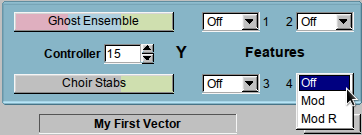
\includegraphics[scale=0.75]{1.4.0/yoshimi-vectors-feature-4.png}
   \caption{Yoshimi Vectors, Feature 4}
   \label{fig:yoshimi_vectors_feature_4}
\end{figure}

   Values: \texttt{Off*, Mod, Mod R}

   \itempar{X Vector}{Vectors!x}
   The X Vector.
   This vector provides the maximal setup for a vector.  This setup requires
   \textsl{Yoshimi} to be configured for 64 parts, to be able to fully support
   an additional two-part vector for every MIDI channel.  This section is
   disabled until selects a \textbf{Controller} event value for it.

   Other than that, the \textbf{Y} vector acts like the \textbf{X} vector, and
   all of the sub-items have the same functionality as in the
   \textbf{X} vector.

\begin{figure}[H]
   \centering 
   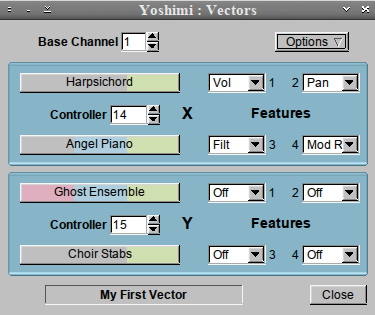
\includegraphics[scale=0.75]{1.4.0/yoshimi-vectors-saved.png}
   \caption{Yoshimi Vectors Saved as "My First Vector"}
   \label{fig:yoshimi_vectors_saved}
\end{figure}

   If starting a new vector setup, first
   select the base channel (1 to 16) to set the vector on. Next,
   use the \textbf{X} and \textbf{Y} \textbf{Controller}
   spin-boxes to select the incoming CC.
   If you set an invalid one strange things may happen, though it won't
   actually do any harm.

   The instrument buttons bring up the instrument list window in exactly the same
   way as the main part one does, but do not currently the right-click
   windows return feature.

   When setting up a completely new vector, if the mixer or the main part are
   visible, they may be slightly out of sync, but will correct themselves as
   soon as one changes an instrument or part.

   When one \textbf{clears} a vector it doesn't delete loaded voices, nor does
   it change the active status of the part, nor the number of parts available.
   This is because these settings may have been made independent of vector
   control. In short, vector setup will add things but not remove them.

\subsection{Vector / Vector Control}
\label{subsection:vector_control}

   Setting up vector control via MIDI is currently done as follows.
   In the required channel send:

   \begin{itemize}
      \item NRPN MSB (99) set to 64
      \item NRPN LSB (98) set to 1 [8192]
      \item Data MSB (6) set mode:
      \begin{itemize}
         \item 0 = X sweep CC
         \item 1 = Y sweep CC
         \item 2 = enable X features
         \item 3 = enable Y features
         \item 4 = x1 instrument (optional)
         \item 5 = x2 instrument (optional)
         \item 6 = y1 instrument (optional)
         \item 7 = y2 instrument (optional)
      \end{itemize}
   \end{itemize}

   Setting CC for X enables vector control; any value outside the above list
   disables it.

   Data LSB (38) value to set features:

   \begin{itemize}
       \item 1 = Volume (fixed)
       \item 2 = Pan (the default)
       \item 4 = Filter Cutoff (Brightness, it is the default)
       \item 8 = Mod Wheel (the default)
       \item 0x12 = 18 = Reversed Pan
       \item 0x24 = 36 = Reversed Filter Cutoff
       \item 0x48 = 72 = Reversed Mod Wheel
   \end{itemize}

   The feature numbers are chosen so they can be combined. So, 5 would be
   Volume + Brightness and 19 would be Volume + Reversed Pan.

   Setting the sweep CC for the X axis enables vector control. It also sets,
   but doesn't enable the default X axis features.  Setting the sweep CC for
   the Y axis sets, but doesn't enable the default Y axis features.  If one
   doesn't enable any features, not a lot will happen.

   The feature numbers are chosen so they can be combined. So, 5 would be
   Volume + Brightness and 19 would be Volume + Reversed Pan.

   Optional settings.  The first part, the number, is the MSB value.
   The second part is the LSB, the parameter value to set.  Note that the
   instrument IDs are for instruments in the current bank.

   \begin{itemize}
      \item 4 = x1 instrument ID
      \item 5 = x2 instrument ID
      \item 6 = y1 instrument ID
      \item 7 = y2 instrument ID
      \item 8 = set CC for X feature 2
      \item 9 = set CC for X feature 4
      \item 10 = set CC for X feature 8
      \item 11 = set CC for Y feature 2
      \item 12 = set CC for Y feature 4
      \item 13 = set CC for Y feature 8
   \end{itemize}
              
   The IDs are for instruments in the current bank.
   Any data MSB value outside the above list disables vector control.
   Sweep CCs and feature CCs are sanity-checked.
    
   An Example. From channel 1, send the following CCs:

   \begin{verbatim}
      CC      Value
      99       64
      98        1
       6        0
      38       14
      98        1 *
       6        1
      38       15
      98        1 *
       6        2
      38        1
      98        1 *
       6        3
      38        2
   \end{verbatim}

   This sequence will set up CC 14 as the X axis incoming controller,
   and CC 15 as the Y axis incoming controller, with X set to volume control
   and Y set to pan control.

   One can either go on with the NRPNs to set the instruments (this will load
   and enable instruments from the current bank), or enable and load
   them by hand.  For channel 1 this would be part 1 and 17 for X and part 33
   and 49 for Y.

   The (*) CCs ensure that the data bytes are reset each time. This is not
   really necessary for the earlier commands, but should be done if one sets
   the instruments with NRPNs as well, otherwise one will try to set them
   twice.

\subsection{Vector / Command Line}
\label{subsection:vector_command_line}

   This section covers material that could be in the command-line section
   (see \sectionref{sec:command_line}), but is really too detailed to cover
   there.  The examples here, to set up vectors from the command line,
   are provided by Will.

   Assuming we want just a single axis on channel 1 (which is channel
   2 in the GUI), first we need to make sure we have enough parts available:

   \begin{verbatim}
      yoshimi> set available 32
      Available parts set to 32
   \end{verbatim}

   The next command must aways be the first command, as everthing else depends
   on it. It's the command that \textsl{enables} vector control.  The
   \texttt{x} token denotes the "x axis", and the \texttt{cc} token, followed
   by 14, is the incoming sweep CC (control change) that will vary the
   features one sets.

   \begin{verbatim}
      yoshimi > set vector 1 x cc 14
      Vector channel set to 1
   \end{verbatim}

   Note that, according to the list of MIDI CC's at
   \url{http://nickfever.com/music/midi-cc-list}, CC 14 is undefined,
   normally.  It is thus available for \textsl{Yoshimi} to assign
   for its own purpose.

   \index{vector!features}
   There are four vector features currently available:

   \index{vector!1 volume}
   \index{vector!2 pan}
   \index{vector!3 brightness}
   \index{vector!4 modulation}
   \begin{itemize}
      \item \textbf{1} is fixed as \textsl{volume}.
      \item \textbf{2} is \textsl{pan} by default.
      \item \textbf{3} is \textsl{brightness} by default.
      \item \textbf{4} is \textsl{modulation} by default.
   \end{itemize}

   We will select \textsl{volume} for this example.  Let's enable this
   feature:

   \begin{verbatim}
      yoshimi Vect Ch 1 X > set features 1 enable
      Set X features 1 en
   \end{verbatim}

   Next, one needs to set the instruments that will be used.
   The instruments can only be selected from the instruments
   in the current bank. Therefore, assuming the current bank is
   the "\textsl{Will Godfrey Companion}", let's set up two instruments:

   \begin{verbatim}
      yoshimi Vect Ch 1 X > set program left 20
      Loaded 20 "Bubbles" to Part 1

      yoshimi Vect Ch 1 X > set program right 120
      Loaded 120 "Ghost Ensemble" to Part 16
   \end{verbatim}

   The \texttt{left} token merely assigns instrument 20 to a "virtual"
   left side of the X axis,
   and the \texttt{right} token assigns instrument 20 to a "virtual"
   right side of the X axis.

   \textsl{(Chris asks:  How did the part numbers 1 and 16 come about? What
   are the rules?  Why are 32 parts needed, if only 1 to 16 are involved?  Why
   do we need to have 64 parts when we add the Y axis below?  Can we set
   intermediate values between "left" and "right" and "up" and "down" to
   get some really weird morphs?)}

   \index{vector!morph}
   If one now sweeps the the controller assigned to CC 14,
   the sound will morph between these two instruments.

   To continue on to using the other axis as well, one needs to have 64 parts
   available:

   \begin{verbatim}
      yoshimi Vect Ch 1 X > /set available 64
      Available parts set to 64
   \end{verbatim}

   \index{command level}
   Note the slash, which lets the user immediately access the topmost command
   level, where the "available parts" setting can be performed.
   Then:

   \begin{verbatim}
      yoshimi > set vector y cc 15
      Vector 1 Y CC set to 15
   \end{verbatim}

   This command sets up the Y axis to be controlled by MIDI CC 15, which is,
   again, a CC that is normally undefined.
   We will use \textsl{panning} (feature 2) for this vector, which is defined
   on the Y axis:

   \begin{verbatim}
      yoshimi Vect Ch 1 Y > set features 2 enable
      Set Y features 2 en
   \end{verbatim}

   Analogous to the "left" and "right" virtual directions used above for the X
   axis, the Y axis used the "up" and "down" virtual directions:

   \begin{verbatim}
      yoshimi Vect Ch 1 Y > set program down 107
      Loaded 107 "Angel Harp" to Part 32

      yoshimi Vect Ch 1 Y > set program up 78
      Loaded 78 "Brassy Flutter" to Part 48
   \end{verbatim}

   Notice that the directions left, right, up, and down match the directions
   provided by a traditional joystick.

   So we have now set up a vector sound where MIDI CC 14 morphs the sound
   through a continuous linear combination of two different instruments,
   and MIDI CC 15 morphs the sound between two other instruments.
   One can then save one's cool vector sound to a file:

   \begin{verbatim}
      yoshimi Vect Ch 1 Y > save vector CoolSound
      Saved channel 1 Vector to CoolSound
   \end{verbatim}

   The file extension for the save vector sound file is \texttt{.xvy}, and
   this extension is added automatically.  The final name of the file is
   \texttt{CoolSound.xvy}.

   \textsl{(Chris asks:  Where is this file saved?  Is there a way to modify
   this location?)}

   At any time one can reload this vector sound file from the command-line:

   \begin{verbatim}
      yoshimi> load vector channel 0 CoolSound
      Loaded Vector CoolSound to channel 0
   \end{verbatim}

   If there is no channel number provided, then the vector sound
   will be loaded to the same channel as it was saved from:

   \begin{verbatim}
      yoshimi> load vector CoolSound
      Loaded Vector CoolSound to source channel
   \end{verbatim}

%-------------------------------------------------------------------------------
% vim: ts=3 sw=3 et ft=tex
%-------------------------------------------------------------------------------
